$subject$=Теория вероятности
$date$=03.12.2024
$teacher$=Лекции Блаженова А. В.

\section{Лекция 14}

\subsection{Пространство случайных величин}

\begin{minipage}{\textwidth}
    \begin{wrapfigure}{r}{0pt}
        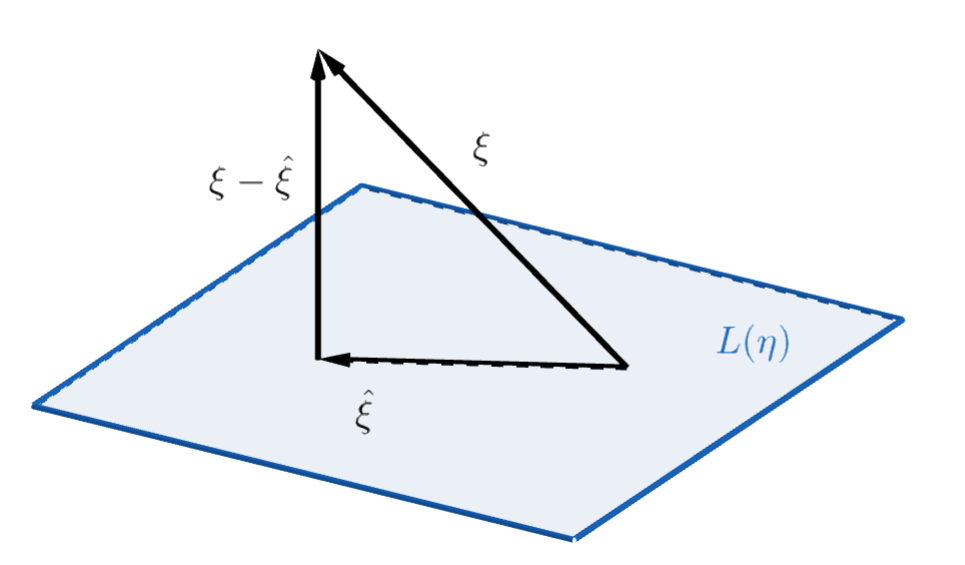
\includegraphics[width=5cm]{probtheory/images/probtheory_2024_12_03_1}
    \end{wrapfigure}

    \Nota Если две случайных величин $\xi \overset{\text{п.н.}}{=} \eta$, то считаем, что $\xi = \eta$

    Пусть имеется вероятностное пространство $(\Omega, \mathcal{F}, P)$

    Введем пространство $L_2 (\Omega, \mathcal{F}, P) = \{\xi \ | \ D\xi < \infty\}$ - множество случайных величин 
    на данном пространстве с конечной дисперсией

    Ясно, что $L_2$ - линейное пространство. Введем на нем скалярное произведение

    \Def Скалярным произведением случайных величин $\xi$ и $\eta$ из $L_2(\Omega, \mathcal{F}, P)$ 
    называется число $(\xi, \eta) = E(\xi\eta)$

    \Nota Если $(\xi, \eta)$ - дискретная система случайных величин ($p(\xi = x_i, \eta = y_i) = p_{ij}$), 
    то $E(\xi\eta) = \sum_{i, j} x_i y_j p_{ij}$
\end{minipage}

Если же $(\xi, \eta)$ - непрерывная система с плотностью $f_{\xi, \eta}(x, y)$, 
то $E(\xi\eta) = \iint_{\Real^2} xy f_{\xi, \eta}(x, y) dxdy$

\mediumvspace

\textbf{Свойства}:

\begin{enumerate}
    \item $(\xi, \eta) = (\eta, \xi)$

    \item $(C\xi, \eta) = C(\xi, \eta)$

    \item $(\xi_1 + \xi_2, \eta) = (\xi_1, \eta) + (\xi_2, \eta)$

    \item $(\xi, \xi) \geq 0$

    \item $(\xi, \xi) = 0 \Longrightarrow \xi = 0$ п.н.
\end{enumerate}

То есть это действительно скалярное произведение

\Def Норма вектора равна числу $\|\xi\| = \sqrt{(\xi, \xi)}$

\Def Метрикой (расстоянием) между случайными величинами называют число $d(\xi, \eta) = \|\xi - \eta\|$

\begin{MyTheorem}
    \Ths Неравенство Коши-Буняковского-Шварца

    Пусть случайные величины $\xi$ и $\eta$ имеют конечный второй момент, тогда 
    $|E(\xi, \eta)| \leq \sqrt{E\xi^2 \cdot E\eta^2}$ (или $|(\xi, \eta)| \leq \|\xi\|\cdot\|\eta\|$)

    Причем $|E(\xi, \eta)| = \sqrt{E\xi^2 \cdot E\eta^2} \Longleftrightarrow \eta = C\xi$, где $C = \mathrm{const}$
\end{MyTheorem}

\begin{MyProof}
    $P_2(x) = E(x\xi - \eta)^2 = x^2 E\xi^2 - 2xE(\xi\eta) + E\eta^2 \geq 0 \Longrightarrow D = 4(E(\xi\eta))^2 - 
    4 E\xi^2 - E\eta^2 \leq 0 \Longrightarrow |E(\xi\eta)| \leq \sqrt{E\xi^2 \cdot E\eta^2}$
    
    $|E(\xi, \eta)| = \sqrt{E\xi^2 - E\eta^2} \Longrightarrow D = 0 \Longrightarrow \exists$ какая-либо точка касания $C$, 
    из этого $E(C\xi - \eta)^2 = 0 \Longrightarrow C\xi - \eta = 0 \Longleftrightarrow \eta = C\xi \text{ п.н. }$
\end{MyProof}

\subsection{Условное математическое ожидание}

В $L_2(\Omega, \mathcal{F}, P)$ возьмем линейное подпространство $L(\eta) = \{g(\eta) \ | \ Dg(\eta) < \infty\}$

\DefN{B} Условное математическое ожидание (УМО, обозначается $E(\xi|\eta) = \hat{\xi}$) случайной величины $\xi$
относительно случайной величины $\eta$ называется ортогональная проекция случайной величины $\xi$ на $L(\eta)$ 

\mediumvspace

\textbf{Свойства}:

\begin{enumerate}

    \item Тождество ортопроекций: $\letsymbol \hat{\xi} \in L(\eta)$, тогда $\hat{\xi} = E(\xi|\eta) \Longleftrightarrow E(\xi\cdot g(\eta)) = E(\hat{\xi}\cdot g(\eta)) \ \forall g(\eta) \in L(\eta)$

    \begin{MyProof}
        $\hat{\xi} = E(\xi|\eta) \Longleftrightarrow (\xi - \hat{\xi}) \perp L(\eta) \Longleftrightarrow 
        (\xi - \hat{\xi}, g(\eta)) = 0 \ \forall g(n) \in L(\eta) \Longleftrightarrow E(\xi\cdot g(\eta)) = E(\hat{\xi}\cdot g(\eta))$
    \end{MyProof}

    \item Формула полного математического ожидания

    $E\xi = E(E(\xi|\eta))$ или $E\xi = E\hat{\xi}$

    \Nota При распределении Бернулли получаем обычную формулу полной вероятности

    \begin{MyProof}
        Верно из тождества ортопроекций при $g(\eta) = 1$
    \end{MyProof}

    \item Линейность: $E(C_1\xi_1 + C_2\xi_2 \ | \ \eta) = C_1 E(\xi_1|\eta) + C_2 E(\xi_2|\eta)$

    \item Если $\xi$ и $\eta$ независимы, то $E(\xi|\eta) = E\xi$

    \begin{MyProof}
        $\xi, \eta$ независимы $\Longrightarrow \xi$ и $g(\eta)$ независимы

        Из этого $E(\xi \cdot g(\eta)) = E\xi \cdot E(g(\eta)) = E(E\xi \cdot g(\eta)) \Longrightarrow E\xi = \hat{\xi}$
    \end{MyProof}

    \item Если $\xi$ и $\eta$ независимы, то $(\xi - E\xi) \perp g(\eta) \ \forall g(\eta) \in L(\eta)$, 
в частности $(\xi - E\xi) \perp \eta$

\end{enumerate}

Докажем, что \DefN{A} согласуется c \DefNs{B}

По \DefNs{A} $E(\xi|\eta) = h(\eta)$, где $h(y) = E(\xi|\eta = y)$

Рассмотрим случай абсолютно непрерывной системы $(\xi, \eta)$ с плотностью $f_{\xi,\eta}(x, y)$.
Тогда $h(y) = \int_{-\infty}^\infty xf(x|y)dx$, где $f(x|y) = \frac{f_{\xi,\eta}(x, y)}{f_\eta(y)}$

Следует доказать, что функция $h(y)$ удовлетворяет тождеству ортопроекций $E(\xi g(\eta)) = E(h(\eta)g(\eta)) \ \forall g(\eta) \in L(\eta)$

$E(\xi\cdot g(\eta)) = \iint_{\Real^2} xg(y) f_{\xi,\eta}(x, y)dxdy$

$E(h(\eta)g(\eta)) = \int_{-\infty}^{\infty} h(y) g(y) f_{\eta}(y) dy = \int_{-\infty}^\infty \left(\int_{-\infty}^\infty x\frac{f_{\xi,\eta}(x, y)}{f_\eta(y)}dx\right) g(y) f_\eta(y) = dy = \iint_{\Real^2} xg(y)f_{\xi,\eta}(x, y)dxdy = E(\xi g(\eta))$

\subsection{Числовые характеристики. Зависимости случайных величин}

\Mem Если случайные величины $\xi$ и $\eta$, то $E(\xi\eta) = E\xi E\eta \Longrightarrow E(\xi\eta) - E\xi E\eta = 0$

Поэтому в качестве индикатора наличия связи берем величину $E(\xi\eta) - E\xi E\eta = \mathrm{cov}(\xi, \eta)$

\Def Ковариацией $\mathrm{\cov}(\xi, \eta)$ называется величина $\mathrm{cov}(\xi, \eta) = E((\xi - E\xi)(\eta - E\eta))$

\mediumvspace

\textbf{Свойства}:

\begin{enumerate}
    \item $\mathrm{cov} (\xi, \eta) = E(\xi\eta) - E\xi E\eta$

    \begin{MyProof}
        $\mathrm{cov}(\xi, \eta) = E((\xi - E\xi)(\eta - E\eta)) = E(\xi\eta - \eta E\xi - \xi E\eta + E\xi E\eta) = E(\xi\eta) - E\xi E\eta$
    \end{MyProof}

    \item $\mathrm{cov} (\xi, \xi) = D\xi$

    \begin{MyProof}
        $\mathrm{cov}(\xi, \xi) = E\xi^2 - (E\xi)^2$
    \end{MyProof}

    \item $\mathrm{cov}(\xi, \eta) = \mathrm{cov}(\eta, \xi)$

    \item $\mathrm{cov}(C_1 \xi_1 + C_2 \xi_2, \eta) = C_1 \mathrm{cov}(\xi_1, \eta) + C_2 \mathrm{cov}(\xi_2, \eta)$

    \item $D(\xi + \eta) = D\xi + D\eta + 2\mathrm{cov}(\xi, \eta)$

    \item $D(\xi_1 + \dots + \xi_n) = \sum_{i = 1}^n D\xi_i + 2\sum_{i < j} \mathrm{cov}(\xi_i, \xi_j) = \sum_{i, j = 1}^{n} \mathrm{cov}(\xi_i, \xi_j)$

    \item \begin{enumerate}
        \item Если $\xi$ и $\eta$ - независимы, то $\mathrm{cov}(\xi, \eta) = 0$

        \item Если $\mathrm{cov}(\xi, \eta) \neq 0$, то $\xi$ и $\eta$ - зависимы

        \item Если $\mathrm{cov}(\xi, \eta) = 0$, то неясно
    \end{enumerate}

    \item Если $\mathrm{cov}(\xi, \eta) > 0$, то зависимость прямая, если $\mathrm{cov}(\xi, \eta) < 0$, то обратная
\end{enumerate}

\Nota Ковариация зависит от единиц измерения случайных величин, поэтому по ее величине нельзя судить о силе зависимости

\subsection{Коэффициент линейной корреляции}

\Def Коэффициентом корреляции случайных величин $\xi$ и $\eta$ с конечными вторыми моментами,
называется величина $r_{\xi,\eta} = \frac{\mathrm{cov(\xi, \eta)}}{\sqrt{D\xi} \sqrt{D\eta}} = \frac{E(\xi\eta) - E\xiE\eta}{\sigma_\xi \sigma_\eta}$

Можно записать в другой форме: $r_{\xi,\eta} = \frac{E((\xi - E\xi)(\eta - E\eta))}{\sqrt{E(\xi - E\xi)^2}\sqrt{E(\eta - E\eta)^2}} = 
\frac{(\xi - E\xi, \eta - E\eta)}{\|\xi - E\xi\|\|\eta - E\eta\|} = \cos(\widehat{\xi - E\xi, \eta - E\eta})$ - косинус угла между величинами (грубая интерпретация)

\mediumvspace

\textbf{Свойства}:

\begin{enumerate}
    \item $r_{\xi, \eta} = r_{\eta, \xi}$

    \item \begin{enumerate}
        \item Если $\xi$ и $\eta$ - независимы, то $r_{\xi,\eta} = 0$

        \item Если $r_{\xi,\eta} \neq 0$, то $\xi$ и $\eta$ - зависимы

        \item Если $r_{\xi,\eta} = 0$, то неясно
    \end{enumerate}

    \item $|r_{\xi,\eta}| \leq 1$

    \begin{MyProof}
        По неравенству Коши-Буняковского-Шварца $|E((\xi - E\xi)(\eta - E\eta))| \leq \sqrt{E(\xi - E\xi)^2 E(\eta - E\eta)^2}$
    \end{MyProof}

    \item $|r_{\xi,\eta}| = 1 \Longleftrightarrow \eta = a \xi + b$ п.н.

    \begin{MyProof}
        По неравенству Коши-Буняковского-Шварца $|r_{\xi,\eta}| = 1 \Longleftrightarrow 
        |E((\xi - E\xi)(\eta - E\eta))| = \sqrt{E(\xi - E\xi)^2 E(\eta - E\eta)^2} \Longrightarrow \eta - E\eta = C(\xi - E\xi) \Longrightarrow \eta = C\xi + (E\eta - CE\xi)$ п.н.
    \end{MyProof}

    \item \begin{enumerate} 
        \item Если $r_{\xi,\eta} = 1$, то $\eta = a\xi + b$ и $a > 0$ (прямая линейная зависимость)

        \item Если $r_{\xi,\eta} = -1$, то $\eta = a\xi + b$ и $a < 0$ (обратная линейная зависимость)
    \end{enumerate}

    \begin{MyProof}
        Так как $|r_{\xi,\eta}| = 1$, то по свойству 4) $\eta = a\xi + b$ и $r_{\xi,\eta} = \frac{E(\xi\eta) - E\xi E\eta}{\sigma_\xi \sigma_\eta} = 
        \frac{E(\xi(a\xi + b)) - E\xi E(a\xi + b)}{\sqrt{D\xi D(a\xi + b)}} = \frac{aE\xi^2 + bE\xi - a(E\xi)^2 - bE\xi}{\sqrt{D\xi a^2 D\xi}} = \frac{a(E\xi^2 - (E\xi)^2)}{|a|D\xi} = \frac{a}{|a|} = \mathrm{sign} \,a$
    \end{MyProof}
\end{enumerate}

\Def Если $r_{\xi,\eta} \neq 0$, то говорят, что случайные величины коррелированы друг с другом. Если $r_{\xi,\eta} > 0$, 
то имеет прямая корреляция, если $r_{\xi,\eta} < 0$ - обратная

\Nota Корреляция не транзитивна: $r_{\xi_1,\xi_2} > 0 \land r_{\xi_2,\xi_3} > 0 \centernot\Longrightarrow r_{\xi_1,\xi_3} > 0$

